\documentclass[tikz,border=50mm]{standalone}
% !TeX program = luatex

%===This is the preambule I call in every file===

\usepackage{tikz}
\usepackage{xcolor}
\usepackage{pgfplots}
\usepackage{circuitikz}
\usepackage{tikz-3dplot}
\pgfplotsset{compat=newest}
\usetikzlibrary{arrows.meta, shapes.geometric, positioning, perspective, patterns.meta, decorations.pathreplacing, decorations.pathmorphing, decorations.markings, patterns, arrows.meta, shapes, shapes.geometric, decorations.text, angles, quotes,calc, 3d, math, circuits.ee.IEC,hobby, knots, intersections, through}


%=== The Euler Med Logo ===
%=== i.e. My signature ===

\usepackage{amsmath, amsfonts}
\makeatletter
\newcommand*\eulermed{{
\scalebox{3.3}{$\mathbb{E}$}\kern-1pt \scalebox{1.5}{u$\ell\varepsilon\rho$}\kern-55pt
\raisebox{19pt}{\scalebox{1.5}{$\mathcal{M}\varepsilon\delta$}}}
\@}
\makeatother

\begin{document}
%the code is a little bit messy because it's old (I'll update this later)
%Adding the following commands gives a cool view (\pagecolor{black}, \color{white} necessitate the xcolor package)
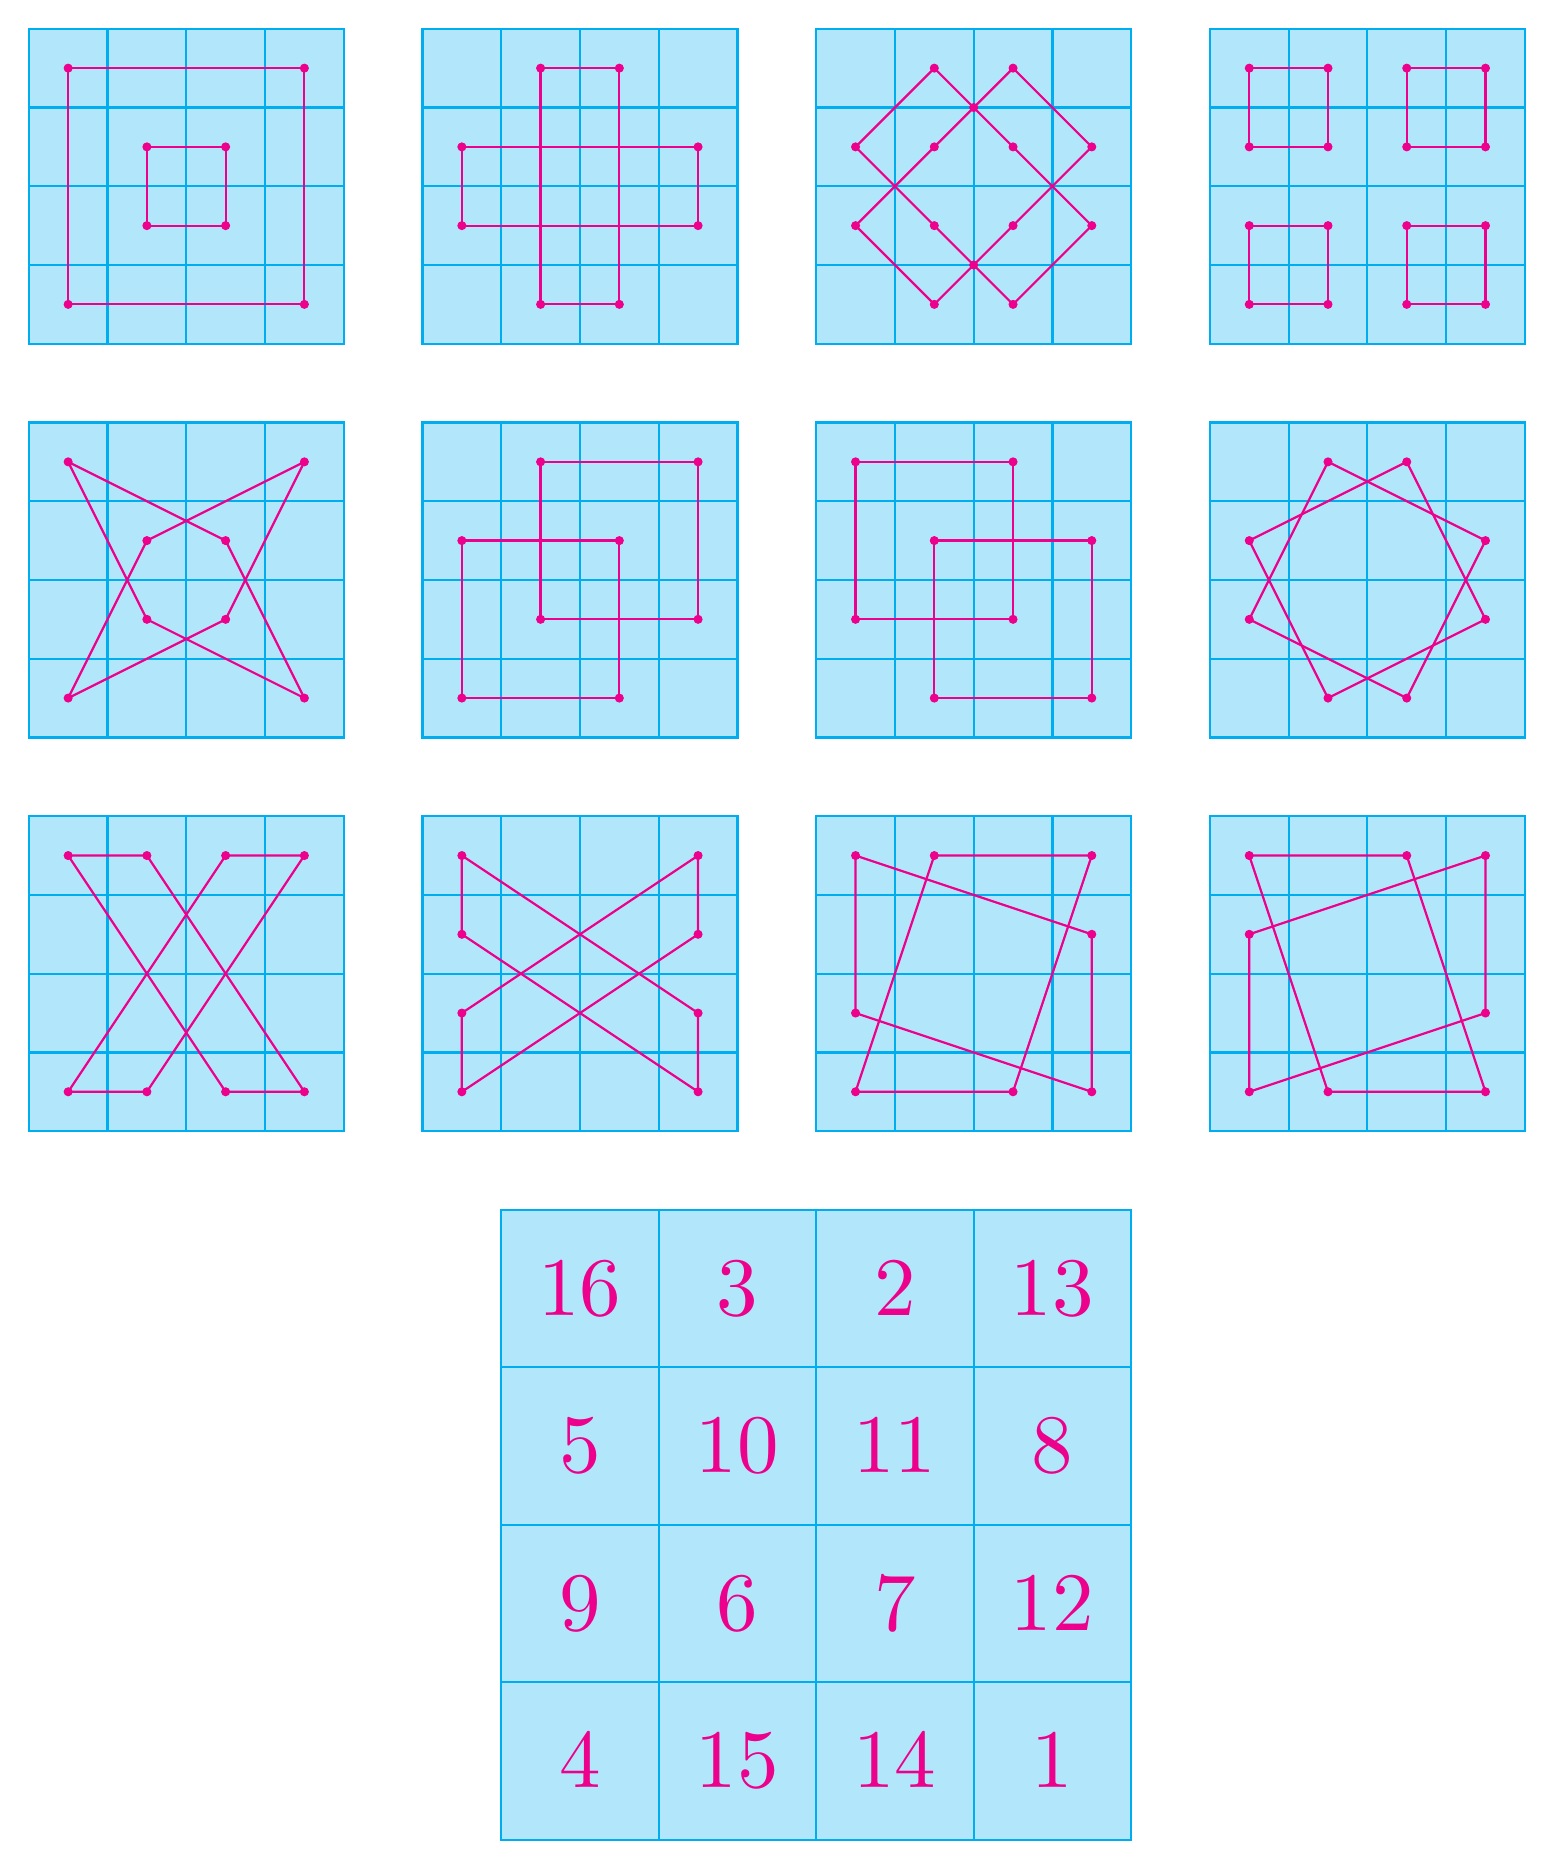
\begin{tikzpicture}
%1st set of squares
\foreach \k in {0, 5, 10, 15}{
\draw[cyan, thick](\k,0)rectangle(\k+4,4); 
\draw[fill=white!90!cyan, opacity=0.3, cyan] (\k,0)rectangle(\k+4,4);
\foreach \i in {\k+1, \k+2, \k+3}{
\draw[thick, cyan] (\i,0)--(\i,4);
}
\foreach \j in {1, 2, 3}{
\draw[thick, cyan] (\k,\j)--(\k+4,\j);
}
}
%1st sums
%first set
\filldraw[magenta] (0.5,3.5)coordinate(c1)circle(0.05);
\filldraw[magenta] (3.5,3.5)coordinate(c2)circle(0.05);
\filldraw[magenta] (3.5,0.5)coordinate(c3)circle(0.05);
\filldraw[magenta] (0.5,0.5)coordinate(c4)circle(0.05);
\draw[magenta, thick] (c1)--(c2)--(c3)--(c4)--cycle;
%second set
\filldraw[magenta] (1.5,2.5)coordinate(c1)circle(0.05);
\filldraw[magenta] (2.5,2.5)coordinate(c2)circle(0.05);
\filldraw[magenta] (2.5,1.5)coordinate(c3)circle(0.05);
\filldraw[magenta] (1.5,1.5)coordinate(c4)circle(0.05);
\draw[magenta, thick] (c1)--(c2)--(c3)--(c4)--cycle;
%2nd set
\begin{scope}[shift={(5,0)}]
%first set
\filldraw[magenta] (1.5,3.5)coordinate(c1)circle(0.05);
\filldraw[magenta] (2.5,3.5)coordinate(c2)circle(0.05);
\filldraw[magenta] (2.5,0.5)coordinate(c3)circle(0.05);
\filldraw[magenta] (1.5,0.5)coordinate(c4)circle(0.05);
\draw[magenta, thick] (c1)--(c2)--(c3)--(c4)--cycle;
%second set
\filldraw[magenta] (0.5,1.5)coordinate(c1)circle(0.05);
\filldraw[magenta] (0.5,2.5)coordinate(c2)circle(0.05);
\filldraw[magenta] (3.5,2.5)coordinate(c3)circle(0.05);
\filldraw[magenta] (3.5,1.5)coordinate(c4)circle(0.05);
\draw[magenta, thick] (c1)--(c2)--(c3)--(c4)--cycle;
\end{scope}
%3rd sums
\begin{scope}[shift={(10,0)}]
%first set
\filldraw[magenta] (0.5,2.5)coordinate(c1)circle(0.05);
\filldraw[magenta] (1.5,3.5)coordinate(c2)circle(0.05);
\filldraw[magenta] (3.5,1.5)coordinate(c3)circle(0.05);
\filldraw[magenta] (2.5,0.5)coordinate(c4)circle(0.05);
\draw[magenta, thick] (c1)--(c2)--(c3)--(c4)--cycle;
%second set
\filldraw[magenta] (0.5,1.5)coordinate(c1)circle(0.05);
\filldraw[magenta] (1.5,0.5)coordinate(c2)circle(0.05);
\filldraw[magenta] (2.5,3.5)coordinate(c3)circle(0.05);
\filldraw[magenta] (3.5,2.5)coordinate(c4)circle(0.05);
\draw[magenta, thick] (c1)--(c2)--(c4)--(c3)--cycle;
\filldraw[magenta] (2,3)coordinate(c1)circle(0.05);
\filldraw[magenta] (2,1)coordinate(c1)circle(0.05);
\filldraw[magenta] (2.5,2.5)coordinate(c1)circle(0.05);
\filldraw[magenta] (1.5,2.5)coordinate(c1)circle(0.05);
\filldraw[magenta] (1.5,1.5)coordinate(c1)circle(0.05);
\filldraw[magenta] (2.5,1.5)coordinate(c1)circle(0.05);
\end{scope}
%4th sums
\begin{scope}[shift={(15,0)}]
%first set
\filldraw[magenta] (2.5,3.5)coordinate(c1)circle(0.05);
\filldraw[magenta] (3.5,3.5)coordinate(c2)circle(0.05);
\filldraw[magenta] (3.5,2.5)coordinate(c3)circle(0.05);
\filldraw[magenta] (2.5,2.5)coordinate(c4)circle(0.05);
\draw[magenta, thick] (c1)--(c2)--(c3)--(c4)--cycle;
%second set
\filldraw[magenta] (0.5,3.5)coordinate(c1)circle(0.05);
\filldraw[magenta] (1.5,3.5)coordinate(c2)circle(0.05);
\filldraw[magenta] (1.5,2.5)coordinate(c3)circle(0.05);
\filldraw[magenta] (0.5,2.5)coordinate(c4)circle(0.05);
\draw[magenta, thick] (c1)--(c2)--(c3)--(c4)--cycle;
%third set
\filldraw[magenta] (0.5,1.5)coordinate(c1)circle(0.05);
\filldraw[magenta] (1.5,1.5)coordinate(c2)circle(0.05);
\filldraw[magenta] (1.5,.5)coordinate(c3)circle(0.05);
\filldraw[magenta] (0.5,.5)coordinate(c4)circle(0.05);
\draw[magenta, thick] (c1)--(c2)--(c3)--(c4)--cycle;
%4th set
\filldraw[magenta] (2.5,1.5)coordinate(c1)circle(0.05);
\filldraw[magenta] (3.5,1.5)coordinate(c2)circle(0.05);
\filldraw[magenta] (3.5,.5)coordinate(c3)circle(0.05);
\filldraw[magenta] (2.5,.5)coordinate(c4)circle(0.05);
\draw[magenta, thick] (c1)--(c2)--(c3)--(c4)--cycle;
\end{scope}
%The 2nd set of squares
\foreach \k in {0, 5, 10, 15}{
\draw[cyan, thick](\k,-5)rectangle(\k+4,-1); 
\draw[fill=white!90!cyan, opacity=0.3, cyan] (\k,-5)rectangle(\k+4,-1);
\foreach \i in {\k+1, \k+2, \k+3}{
\draw[thick, cyan] (\i,-5)--(\i,-1);
}
\foreach \j in {-4, -3, -2}{
\draw[thick, cyan] (\k,\j)--(\k+4,\j);
}
}

\begin{scope}[shift={(0,-5)}]
%First sums 
%1st set
\filldraw[magenta] (.5,3.5)coordinate(c1)circle(0.05);
\filldraw[magenta] (2.5,2.5)coordinate(c2)circle(0.05);
\filldraw[magenta] (3.5,.5)coordinate(c3)circle(0.05);
\filldraw[magenta] (1.5,1.5)coordinate(c4)circle(0.05);
\draw[magenta, thick] (c1)--(c2)--(c3)--(c4)--cycle;
%2nd set
\filldraw[magenta] (3.5,3.5)coordinate(c1)circle(0.05);
\filldraw[magenta] (2.5,1.5)coordinate(c2)circle(0.05);
\filldraw[magenta] (.5,.5)coordinate(c3)circle(0.05);
\filldraw[magenta] (1.5,2.5)coordinate(c4)circle(0.05);
\draw[magenta, thick] (c1)--(c2)--(c3)--(c4)--cycle;
%2nd sums
\begin{scope}[shift={(5,0)}]
%first set
\filldraw[magenta] (.5,2.5)coordinate(c1)circle(0.05);
\filldraw[magenta] (2.5,2.5)coordinate(c2)circle(0.05);
\filldraw[magenta] (2.5,0.5)coordinate(c3)circle(0.05);
\filldraw[magenta] (.5,0.5)coordinate(c4)circle(0.05);
\draw[magenta, thick] (c1)--(c2)--(c3)--(c4)--cycle;
%second set
\filldraw[magenta] (1.5,3.5)coordinate(c1)circle(0.05);
\filldraw[magenta] (3.5,3.5)coordinate(c2)circle(0.05);
\filldraw[magenta] (3.5,1.5)coordinate(c3)circle(0.05);
\filldraw[magenta] (1.5,1.5)coordinate(c4)circle(0.05);
\draw[magenta, thick] (c1)--(c2)--(c3)--(c4)--cycle;
\end{scope}
%3rd sums
\begin{scope}[shift={(10,0)}]
%1st set
\filldraw[magenta] (.5,3.5)coordinate(c1)circle(0.05);
\filldraw[magenta] (2.5,3.5)coordinate(c2)circle(0.05);
\filldraw[magenta] (2.5,1.5)coordinate(c3)circle(0.05);
\filldraw[magenta] (.5,1.5)coordinate(c4)circle(0.05);
\draw[magenta, thick] (c1)--(c2)--(c3)--(c4)--cycle;
%2nd set
\filldraw[magenta] (1.5,2.5)coordinate(c1)circle(0.05);
\filldraw[magenta] (3.5,2.5)coordinate(c2)circle(0.05);
\filldraw[magenta] (3.5,.5)coordinate(c3)circle(0.05);
\filldraw[magenta] (1.5,.5)coordinate(c4)circle(0.05);
\draw[magenta, thick] (c1)--(c2)--(c3)--(c4)--cycle;
\end{scope}
%4th sums
\begin{scope}[shift={(15,0)}]
%first set
\filldraw[magenta] (.5,2.5)coordinate(c1)circle(0.05);
\filldraw[magenta] (2.5,3.5)coordinate(c2)circle(0.05);
\filldraw[magenta] (3.5,1.5)coordinate(c3)circle(0.05);
\filldraw[magenta] (1.5,.5)coordinate(c4)circle(0.05);
\draw[magenta, thick] (c1)--(c2)--(c3)--(c4)--cycle;
%second set
\filldraw[magenta] (1.5,3.5)coordinate(c1)circle(0.05);
\filldraw[magenta] (3.5,2.5)coordinate(c2)circle(0.05);
\filldraw[magenta] (2.5,.5)coordinate(c3)circle(0.05);
\filldraw[magenta] (.5,1.5)coordinate(c4)circle(0.05);
\draw[magenta, thick] (c1)--(c2)--(c3)--(c4)--cycle;
\end{scope}
\end{scope}

%The third set of squares
\foreach \k in {0, 5, 10, 15}{
\draw[cyan, thick](\k,-10)rectangle(\k+4,-6); 
\draw[fill=white!90!cyan, opacity=0.3, cyan] (\k,-10)rectangle(\k+4,-6);
\foreach \i in {\k+1, \k+2, \k+3}{
\draw[thick, cyan] (\i,-10)--(\i,-6);
}
\foreach \j in {-9, -8, -7}{
\draw[thick, cyan] (\k,\j)--(\k+4,\j);
}
}
\begin{scope}[shift={(0,-10)}]
%1st sums
%1st set 
\filldraw[magenta] (.5,3.5)coordinate(c1)circle(0.05);
\filldraw[magenta] (1.5,3.5)coordinate(c2)circle(0.05);
\filldraw[magenta] (3.5,.5)coordinate(c3)circle(0.05);
\filldraw[magenta] (2.5,.5)coordinate(c4)circle(0.05);
\draw[magenta, thick] (c1)--(c2)--(c3)--(c4)--cycle;
%2nd set
\filldraw[magenta] (2.5,3.5)coordinate(c1)circle(0.05);
\filldraw[magenta] (3.5,3.5)coordinate(c2)circle(0.05);
\filldraw[magenta] (1.5,.5)coordinate(c3)circle(0.05);
\filldraw[magenta] (.5,.5)coordinate(c4)circle(0.05);
\draw[magenta, thick] (c1)--(c2)--(c3)--(c4)--cycle;
%2nd sums
\begin{scope}[shift={(5,0)}]
%1st set
\filldraw[magenta] (.5,3.5)coordinate(c1)circle(0.05);
\filldraw[magenta] (.5,2.5)coordinate(c2)circle(0.05);
\filldraw[magenta] (3.5,.5)coordinate(c3)circle(0.05);
\filldraw[magenta] (3.5,1.5)coordinate(c4)circle(0.05);
\draw[magenta, thick] (c1)--(c2)--(c3)--(c4)--cycle;
%2nd set 
\filldraw[magenta] (3.5,3.5)coordinate(c1)circle(0.05);
\filldraw[magenta] (3.5,2.5)coordinate(c2)circle(0.05);
\filldraw[magenta] (.5,.5)coordinate(c3)circle(0.05);
\filldraw[magenta] (.5,1.5)coordinate(c4)circle(0.05);
\draw[magenta, thick] (c1)--(c2)--(c3)--(c4)--cycle;
\end{scope}
%3rd sums
\begin{scope}[shift={(10,0)}]
%1st set 
\filldraw[magenta] (1.5,3.5)coordinate(c1)circle(0.05);
\filldraw[magenta] (3.5,3.5)coordinate(c2)circle(0.05);
\filldraw[magenta] (2.5,.5)coordinate(c3)circle(0.05);
\filldraw[magenta] (.5,.5)coordinate(c4)circle(0.05);
\draw[magenta, thick] (c1)--(c2)--(c3)--(c4)--cycle;
%2nd set
\filldraw[magenta] (.5,3.5)coordinate(c1)circle(0.05);
\filldraw[magenta] (.5,1.5)coordinate(c2)circle(0.05);
\filldraw[magenta] (3.5,.5)coordinate(c3)circle(0.05);
\filldraw[magenta] (3.5,2.5)coordinate(c4)circle(0.05);
\draw[magenta, thick] (c1)--(c2)--(c3)--(c4)--cycle;
\end{scope}
%4th sums
\begin{scope}[shift={(15,0)}]
%the 1st set
\filldraw[magenta] (.5,3.5)coordinate(c1)circle(0.05);
\filldraw[magenta] (2.5,3.5)coordinate(c2)circle(0.05);
\filldraw[magenta] (3.5,.5)coordinate(c3)circle(0.05);
\filldraw[magenta] (1.5,.5)coordinate(c4)circle(0.05);
\draw[magenta, thick] (c1)--(c2)--(c3)--(c4)--cycle;
%the 2nd set
\filldraw[magenta] (.5,2.5)coordinate(c1)circle(0.05);
\filldraw[magenta] (.5,.5)coordinate(c2)circle(0.05);
\filldraw[magenta] (3.5,1.5)coordinate(c3)circle(0.05);
\filldraw[magenta] (3.5,3.5)coordinate(c4)circle(0.05);
\draw[magenta, thick] (c1)--(c2)--(c3)--(c4)--cycle;
\end{scope}
\end{scope}
%The magic square
\begin{scope}[shift={(6,-19)}]
\draw[cyan, thick](0,0)rectangle(8,8); 
\draw[fill=white!90!cyan, opacity=0.3, cyan] (0,0)rectangle(8,8);
\foreach \i in {2,4,6}{
\draw[thick, cyan] (\i,0)--(\i,8);
\draw[thick, cyan] (0,\i)--(8,\i);
}
\node[magenta, scale=3] at (7,1) {1};
\node[magenta, scale=3] at (5,7) {2};
\node[magenta, scale=3] at (3,7) {3};
\node[magenta, scale=3] at (1,1) {4};
\node[magenta, scale=3] at (1,5) {5};
\node[magenta, scale=3] at (3,3) {6};
\node[magenta, scale=3] at (5,3) {7};
\node[magenta, scale=3] at (7,5) {8};
\node[magenta, scale=3] at (1,3) {9};
\node[magenta, scale=3] at (3,5) {10};
\node[magenta, scale=3] at (5,5) {11};
\node[magenta, scale=3] at (7,3) {12};
\node[magenta, scale=3] at (7,7) {13};
\node[magenta, scale=3] at (5,1) {14};
\node[magenta, scale=3] at (3,1) {15};
\node[magenta, scale=3] at (1,7) {16};
\end{scope}
\end{tikzpicture}
\end{document}
